\subsection{多面角的性质}\label{subsec:3-2}

在研究多面角的性质之前,先研究三面角的一个性质:

\begin{dingli}[定理][smj-lgmjh]
    三面角的任意两个面角的和大于第三个面角。
\end{dingli}

已知:三面角 $S{-}ABC$(图 \ref{fig:ltjh-3-4})。

求证:$\angle ASB + \angle BSC > \angle ASC$。

证明:当 $\angle ASC \leqslant \angle ASB$ 时,显然,$\angle ASB + \angle BSC > \angle ASC$。

现在设 $\angle ASC > \angle ASB$。在面 $ASC$ 上作线段 $SD'$,使 $\angle ASD' = \angle ASB$,
过点 $D'$ 引与各棱都相交的平面 $A'B'C'$,使 $SB' = SD'$。这时
$$ \triangle A'SB' \quandeng \triangle A'SD' \douhao $$

$\therefore$ \quad $A'B' = A'D'$。

在 $\triangle A'B'C'$ 中,$A'B' + B'C' > A'C'$,同时 $A'D' + D'C' = A'C'$, 由此得到 $B'C' > D'C'$。

在 $\triangle B'SC'$ 和 $\triangle D'SC'$ 中,因 $B'C' > D'C'$,由余弦定理得 $\cos B'SC' < \cos D'SC'$,

所以 \quad $\angle B'SC' > \angle D'SC'$,即 $\angle BSC > \angle D'SC$。

因此 \quad $\angle ASB + \angle BSC > \angle ASD' + \angle D'SC$,

就是 \quad $\angle ASB + \angle BSC > \angle ASC$。

\begin{figure}[htbp]
    \centering
    \begin{minipage}[b]{7cm}
        \centering
        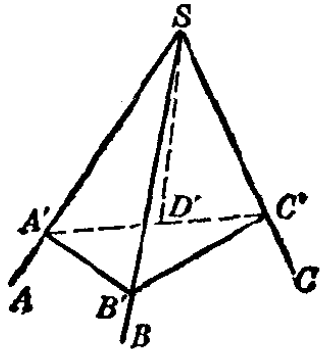
\includegraphics[width=5cm]{../pic/ltjh-ch3-04.png}
        \caption{}\label{fig:ltjh-3-4}
    \end{minipage}
    \qquad \qquad
    \begin{minipage}[b]{7cm}
        \centering
        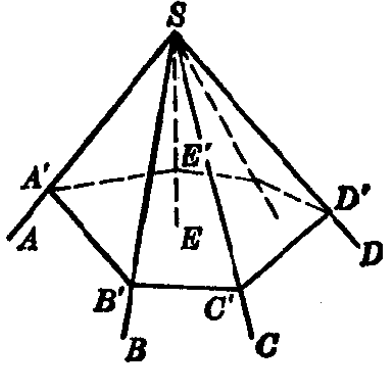
\includegraphics[width=5cm]{../pic/ltjh-ch3-05.png}
        \caption{}\label{fig:ltjh-3-5}
    \end{minipage}
\end{figure}

这里我们注意到,如果使三面角的面与三角形的边对应,三面角的二面角与三角形的内角对应,
那么三面角的一些性质与三角形类似。因此,有些三面角的问题,常归结为三角形的问题来研究。

多面角有下面的性质:

\begin{dingli}[定理][dl:tdmj-symjh]
    凸多面角所有面角的和小于四直角。
\end{dingli}

已知:凸 $n$ 面角 $S{-}ABC{…}E$(图 \ref{fig:ltjh-3-5})。

求证:$\angle ASB + \angle BSC + \cdots + \angle ESA < 4 \cdot Rt \angle$。

证明:用平面截已知多面角的所有面和棱,得到凸 $n$ 边形 $A'B'C'\cdots E'$。
根据前面的定理,以 $A'$、$B'$、$C'$、…、$E'$ 为顶点的各三面角的面角有下面关系:

$\angle SA'E'+ \angle SA'B' > \angle E'A'B'$,

$\angle SB'A' + \angle SB'C' >\angle A'B'C'$,

$\angle SC'B' + \angle SC'D' > \angle B'C'D'$。

…………………………………

用 $\sum$ 表示已知多面角所有面角的和,
$$ {\textstyle\sum} = \angle ASB + \angle BSC + \cdots + \angle ESA \juhao $$

将上面各不等式两边分别相加,左边是 $n$ 个三角形: $\triangle A'SB'$、$\triangle B'SC'$、…、$\triangle E'SA'$
内角的和 $2n \cdot Rt \angle$ 减去已知多面角所有面角的和 $\sum$;
右边是凸多边形 $A'B'\cdots E'$ 所有内角的和,它等于 $2(n - 2) \cdot Rt \angle$,因此,
$$ 2n \cdot Rt \angle - {\textstyle\sum}  > 2(n - 2) \cdot Rt \angle \douhao $$
即 \hspace{18em} $\sum < 4 \cdot Rt \angle$。

这个定理表明,如果沿凸多面角的一个棱剪开,把它展在平面上,那么它不能铺满一个周角,而是缺少一部分(图 \ref{fig:ltjh-3-6})。

\begin{figure}[htbp]
    \centering
    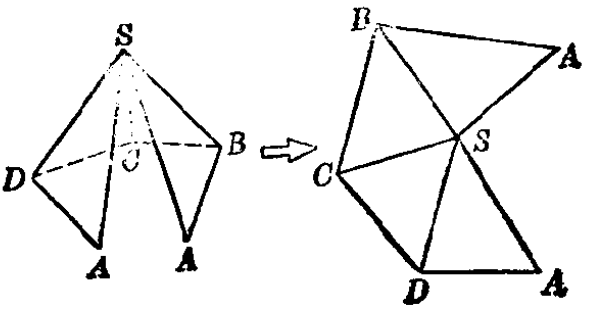
\includegraphics[width=10cm]{../pic/ltjh-ch3-06.png}
    \caption{}\label{fig:ltjh-3-6}
\end{figure}


\begin{lianxi}

\xiaoti{下列各组面角能否构成三面角?为什么?}
\begin{xiaoxiaotis}

    \xxt{$45^\circ$、 $65^\circ$、 $120^\circ$;}

    \xxt{$100^\circ$、 $90^\circ$、 $150^\circ$。}

\end{xiaoxiaotis}

\xiaoti{下列各组面角能否构成四面角?为什么?}
\begin{xiaoxiaotis}

    \xxt{ $45^\circ$, $60^\circ$、 $120^\circ$、 $95^\circ$;}

    \xxt{ $75^\circ$、 $105^\circ$、 $120^\circ$、 $60^\circ$。}

\end{xiaoxiaotis}

\xiaoti{证明:三面角的任何一个面角大于其他两个面角的差。}

\end{lianxi}
